\documentclass{article}
\author{Victor Mittermair, 11809916}
\usepackage{hyperref}
\usepackage{fancyhdr}
\usepackage{tikz} 
\usepackage{amsthm}
\usepackage{verbatim}
\usepackage{subfigure}
\usepackage{amssymb}
\usepackage{mathtools}
\usepackage{amsmath}
\usepackage{soul}
\usepackage{algorithm}
\usepackage{algpseudocode}
\usepackage{algorithmicx}

\newtheorem*{theorem}{Theorem}
\newtheorem*{lemma}{Lemma}
\theoremstyle{definition}
\newtheorem*{definition}{Definition}
\theoremstyle{remark}
\newtheorem*{remark}{Remark}
\newtheorem*{note}{Note}
\newtheorem*{statement}{Statement}
\newtheorem*{example}{Example}

%\lhead{\includegraphics[width=0.2\textwidth]{nyush-logo.pdf}}
\fancypagestyle{firstpage}{%
  \lhead{TU Vienna}
  \rhead{
  Discrete Math for Informatics WS 2022}
}

%%%% PROJECT TITLE
\title{Discrete Math for Informatics\\
        \Large \emph{2nd Lecture}}


\date{\today} %NO DATE



\begin{document}
\maketitle
\thispagestyle{firstpage}


\begin{comment}
\section*{Graph}
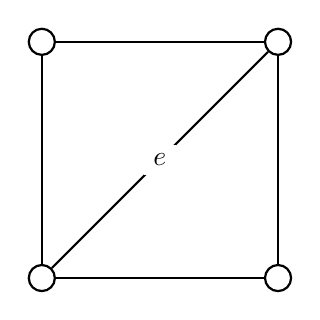
\begin{tikzpicture}[node distance={30mm}, thick, main/.style = {draw, circle}]
    \centering
    \node[main] (1)              {}; 
    \node[main] (2) [right of=1] {};
    \node[main] (3) [below of=1] {}; 
    \node[main] (4) [right of=3] {};
    \draw (1) -- (2) ; 
    \draw (1) -- (3); 
    \draw (2) -- (4); 
    \draw (3) -- (4);
    \draw (3) -- (2) node [midway, fill=white] {$e$}; 
\end{tikzpicture}


\begin{equation}
    \sum_{n = 1}^{\infty} 2n \approx \int_{a}^{b} 2x \,dx 
\end{equation}

\begin{proof}
    Lorem ipsum
\end{proof}

\begin{remark}
    Lorem ipsum
\end{remark}

\begin{definition}[Walk]
    Lorem ipsum
\end{definition}

\begin{theorem}
    Lorem ipsum.
\end{theorem}

\begin{lemma}[Handshake-lemma]
    Lorem ipsum.
\end{lemma}
\end{comment}

\begin{definition}
    An \textbf{Eulerian Trail} is a trail that uses \textbf{every} edge exactly once.
\end{definition}
\begin{theorem}
    A connected graph has a Eulerian circuit if and only if all its vertices have even degree.
\end{theorem}
\begin{figure}[h!]
    \centering
    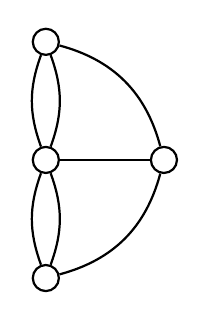
\begin{tikzpicture}[node distance={15mm}, thick, main/.style = {draw, circle}]
        \centering
        \node[main] (1)              {}; 
        \node[main] (2) [below of=1] {};
        \node[main] (3) [below of=2] {}; 
        \node[main] (4) [right of=2] {};
        \draw [bend left=20]  (1) edge (2)  ; 
        \draw [bend left=20] (2) edge (1) ; 
        \draw [bend left=30] (1) edge (4); 
        \draw [bend left=30] (4) edge (3); 
        \draw [bend left=20] (2) edge (3); 
        \draw [bend left=20] (3) edge (2); 
        \draw [bend left=0] (2) edge (4);
    \end{tikzpicture}
    \caption{no eulerian circuit as every vertex has odd degree}
\end{figure}
\begin{proof}
    $\Rightarrow$ in any circuit every vertex is entered as often as it serves as a point of departure.\\
    $\Leftarrow$ induction on the number of edges
    \begin{itemize}
        \item if the graph $G$ has no edges $G$ = $(V = {1}, E = \emptyset)$
        \item otherwise let $W$ be any circuit in G ( this exists: start anywhere, choose any edge unused so far, continue until you hit starting vertex)
        \item let $G^\prime = (V(G), E(G)\backslash E(W))$, all vertices in $G^\prime$ have even degree and $G^\prime$ need not be connected.
        \item let $G^\prime_1, ... G^\prime_c$ be the connected components of $G^\prime$. In each component of $G^\prime_i$ find a Eulerian circuit $W_i$. $W_i$ and $W$ have atleast one vertex in common, because $G$ is connected and removing $W$ produces the components.
        \item therefore $W_1, ... W_c$ and $W$ can be combined to a Eulerian circuit. 
    \end{itemize}
\end{proof}

\section*{Trees and forests}
\begin{definition}
    $ $\\
    \begin{itemize}
        \item a \textbf{forest} is a graph without cylces (=acyclic).
        \item a \textbf{tree} is a connected forest.
        \item a \textbf{leaf} is a vertex of degree 1.
    \end{itemize}
\end{definition}
\begin{lemma}
    if $T$ is a tree and has two vertices it has atleast 2 leafs.
\end{lemma}
\begin{proof}
    $V(T) $ and $E(T)$ are finite $\Rightarrow T$ contains a maximal path, an this path has two leafs (because it is maximal).
\end{proof}
\begin{definition}
    A subgraph $H$ of a graph $G$ is \textbf{spanning} if $V(H) = V(G)$.
\end{definition}
\begin{theorem}[A]
    Let $T$ be a graph, then the following are equivalent:
    \begin{enumerate}
        \item $T$ is a tree.
        \item any 2 vertices are connected with a unique path.
        \item $T$ is connected and every edge is a bridge (min. connected).
        \item $T$ has no cycles and adding any edge yields a cycle (maximal acyclic)
    \end{enumerate}
\end{theorem}
\begin{proof}
    $1\Rightarrow 2$ otherwise $T$ would not be connected or $T$ would have a cylce.\\
    $2 \Rightarrow 3$ A unique path from $u$ to $v$ exists, which means every edge has to be a bridge.\\
    $3 \Rightarrow 4$ An edge in a cycle would not be a bridge $\Rightarrow$ $T$ has no cycles, adding an edge would yield a cyle because T is connected.\\
    $4 \rightarrow 1$ adding any edge $(u,v)$ yields a cycle $= T$ is connected.
\end{proof}
\begin{theorem}[B]
    A connected graph $G$ has a spanning tree.
\end{theorem}
\begin{proof}
    As long as there is a non-bridge remove it, and use 3. of Theorem A
\end{proof}

\begin{theorem}[C]
    A graph is a tree if and only if it is connected and $|V| = |E| + 1$.
\end{theorem}
\begin{proof}
    $\Rightarrow$ induction on $|V|: |V| = 1 \surd $\\
    if $|V| \geq  2:$ remove a leaf to obtain $T^\prime$, by induction $|V(T^\prime )|= |V(T)| - 1$ and $|E(T^\prime)| = |E(T)| - 1$\\
    $|V(T)| = |V(T^\prime)| + 1 = |E(T^\prime)| + 1 + 1 = |E(T) + 1|$\\
    $\Leftarrow$ let $T^\prime$ be a spanning tree of $T$\\
    $|V(T^\prime)|=|E(T^\prime)| + 1$\\
    $|V(T)|=|E(T)| + 1$, $|V(T)|=|V(T^\prime)| \Rightarrow |E(T)|=|E(T^\prime)|\Rightarrow T=T^\prime$
\end{proof}
\pagebreak
How many spanning trees are there?
\begin{example}
    \begin{figure}[h!]
            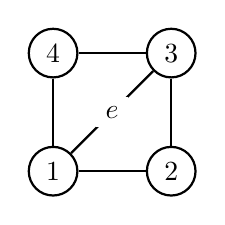
\begin{tikzpicture}[node distance={15mm}, thick, main/.style = {draw, circle}]
                \centering
                \node[main] (1)              {1}; 
                \node[main] (2) [right of=1] {2};
                \node[main] (3) [above of=2] {3}; 
                \node[main] (4) [left of=3] {4};
                \draw  (1) -- (2) ;  
                \draw  (1) -- (3) node [midway, fill=white] {$e$};  
                \draw  (1) edge (4); 
                \draw  (4) edge (3); 
                \draw  (2) edge (3); 
            \end{tikzpicture}
            
    
        \qquad
        \\
        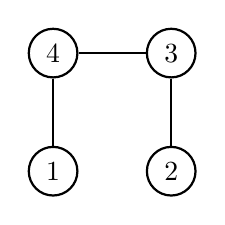
\begin{tikzpicture}[node distance={15mm}, thick, main/.style = {draw, circle}]
            \centering
            \node[main] (1)              {1}; 
            \node[main] (2) [right of=1] {2};
            \node[main] (3) [above of=2] {3}; 
            \node[main] (4) [left of=3] {4};
            \draw  (1) edge (4); 
            \draw  (4) edge (3); 
            \draw  (2) edge (3); 
        \end{tikzpicture}
        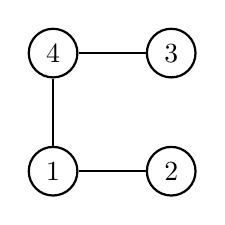
\begin{tikzpicture}[node distance={15mm}, thick, main/.style = {draw, circle}]
            \centering
            \node[main] (1)              {1}; 
            \node[main] (2) [right of=1] {2};
            \node[main] (3) [above of=2] {3}; 
            \node[main] (4) [left of=3] {4};
            \draw  (1) edge (4); 
            \draw  (4) edge (3); 
            \draw  (2) edge (1); 
        \end{tikzpicture}
        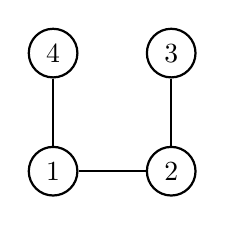
\begin{tikzpicture}[node distance={15mm}, thick, main/.style = {draw, circle}]
            \centering
            \node[main] (1)              {1}; 
            \node[main] (2) [right of=1] {2};
            \node[main] (3) [above of=2] {3}; 
            \node[main] (4) [left of=3] {4};
            \draw  (1) edge (4); 
            \draw  (2) edge (1); 
            \draw  (2) edge (3); 
        \end{tikzpicture}
        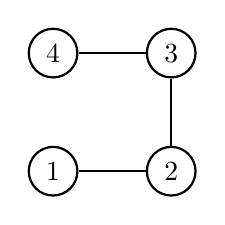
\begin{tikzpicture}[node distance={15mm}, thick, main/.style = {draw, circle}]
            \centering
            \node[main] (1)              {1}; 
            \node[main] (2) [right of=1] {2};
            \node[main] (3) [above of=2] {3}; 
            \node[main] (4) [left of=3] {4};
            \draw  (3) edge (4); 
            \draw  (2) edge (1); 
            \draw  (2) edge (3); 
        \end{tikzpicture}
        \\
        \\
        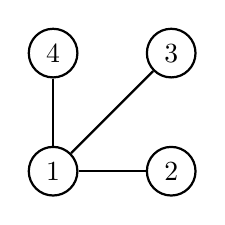
\begin{tikzpicture}[node distance={15mm}, thick, main/.style = {draw, circle}]
            \centering
            \node[main] (1)              {1}; 
            \node[main] (2) [right of=1] {2};
            \node[main] (3) [above of=2] {3}; 
            \node[main] (4) [left of=3] {4};
            \draw  (1) edge (2); 
            \draw  (1) edge (3); 
            \draw  (1) edge (4); 
        \end{tikzpicture}
        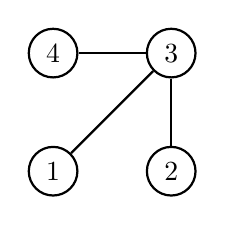
\begin{tikzpicture}[node distance={15mm}, thick, main/.style = {draw, circle}]
            \centering
            \node[main] (1)              {1}; 
            \node[main] (2) [right of=1] {2};
            \node[main] (3) [above of=2] {3}; 
            \node[main] (4) [left of=3] {4};
            \draw  (1) edge (3); 
            \draw  (2) edge (3); 
            \draw  (3) edge (4); 
        \end{tikzpicture}
        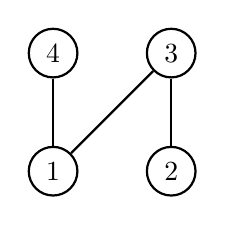
\begin{tikzpicture}[node distance={15mm}, thick, main/.style = {draw, circle}]
            \centering
            \node[main] (1)              {1}; 
            \node[main] (2) [right of=1] {2};
            \node[main] (3) [above of=2] {3}; 
            \node[main] (4) [left of=3] {4};
            \draw  (3) edge (2); 
            \draw  (1) edge (3); 
            \draw  (1) edge (4); 
        \end{tikzpicture}
        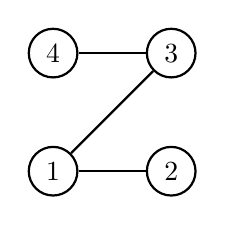
\begin{tikzpicture}[node distance={15mm}, thick, main/.style = {draw, circle}]
            \centering
            \node[main] (1)              {1}; 
            \node[main] (2) [right of=1] {2};
            \node[main] (3) [above of=2] {3}; 
            \node[main] (4) [left of=3] {4};
            \draw  (1) edge (3); 
            \draw  (1) edge (2); 
            \draw  (3) edge (4); 
        \end{tikzpicture}
    \end{figure}
    this graph has 8 spanning trees.
\end{example}
\begin{theorem}[deletion-contraction]
    $\mathcal{T}(G)= \# $ spanning trees.\\
    $G\backslash e ... $ Graph obtained by removing e.\\
    $G / e ...$ Graph obtained by contracting e.\\
    $\mathcal{T}(G) = \mathcal{T}(G\backslash e) + \mathcal{T}(G/e)$
\end{theorem}
\begin{example}
    \begin{equation}
        \mathcal{T}(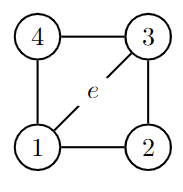
\includegraphics[width=2cm]{G.png}) = \mathcal{T}(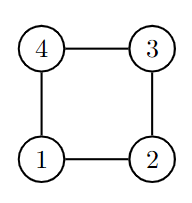
\includegraphics[width=2cm]{G1.png}) + \mathcal{T}(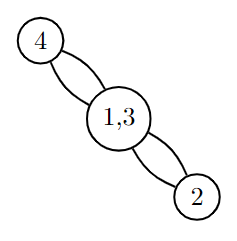
\includegraphics[width=2cm]{G2.png}) = 4 + 4 = 8
    \end{equation}
\end{example}
\begin{proof}
    The set of spanning trees is the disjoint union of spanning trees containing $e$ and spanning trees not containing $e$.
\end{proof}
More generally: if $G$ is a weighted graph with: $w: E(G) \rightarrow  \mathbb{R}$  Let $H$ be a subgraph of G, then $w(H) = \prod_{e \in E(H)} w(e)$\\
$\mathcal{T}(G) $ is the sum of the weights of the spanning tree of $G$\\
\begin{equation}
    \mathcal{T}(G) =  \sum_{T} \prod_{e \in E(T)} w(e)
\end{equation}
\begin{example}
    \begin{equation}
        \mathcal{T}(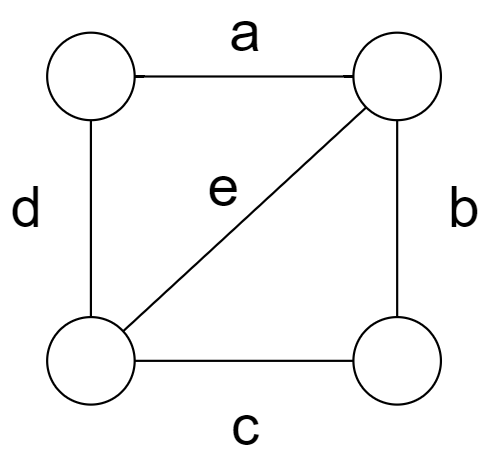
\includegraphics[width=2cm]{1.png}) = \mathcal{T}(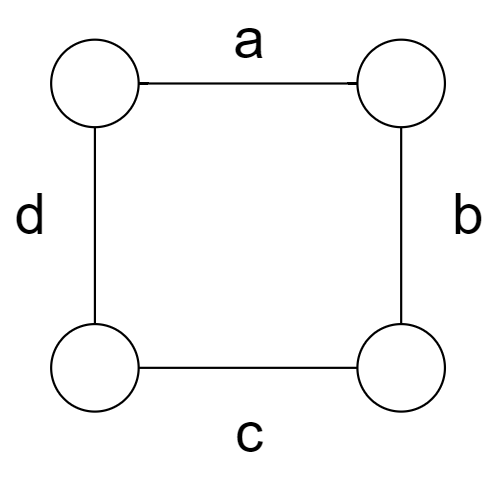
\includegraphics[width=2cm]{2.png}) + e \cdot \mathcal{T}(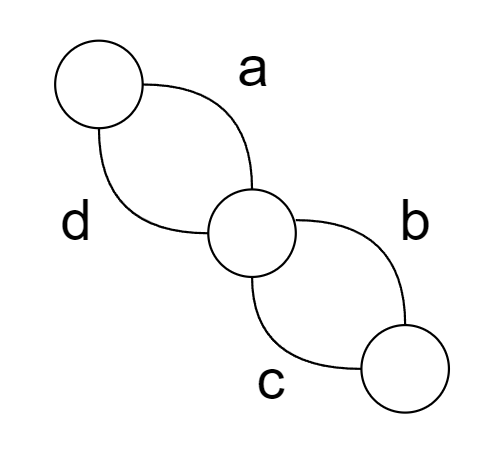
\includegraphics[width=2cm]{3.png}) 
        = abc + abd +acd+bcd+e(a+d)(b+c)
    \end{equation}
\end{example}
\begin{definition}
    The degree matrix of a graph is  $D= $
    \[
        \left(
        \begin{array}{ccccc}
        d(v_1)                                    \\
          & \cdot             &   & \text{\huge0}\\
          &               & \cdot                \\
          & \text{\huge0} &   & \cdot            \\
          &               &   &   & d(v_n)
        \end{array}
        \right)
      \]
   the degree in a weighted graph is $d(u) = \sum_{(u,v) \in E(G)} w(v,u)$
\end{definition}
\begin{theorem}
    Let $n=|V(G)|$ let $\lambda_1,...\lambda_n$ be the eigenvalues of $D-A$. One of these is $0$, w.l.o.g $\lambda_1 = 0$, then $\mathcal{T}(G)=\frac{1}{n} \lambda_2 \cdot ... \cdot \lambda_n$.
    Equivalently: $\mathcal{T}(G) = det((D-A)_{i,i})$ where $M_{i,i}$ is obtained by removing row and column i. $M=D-A$
\end{theorem}
\begin{example}
    \begin{figure}[h!]
        \centering
        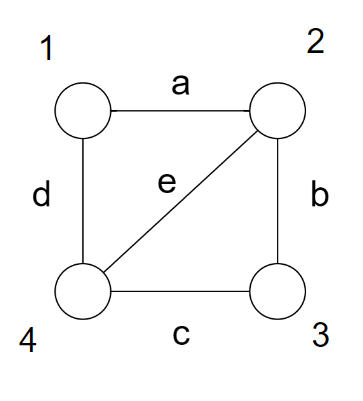
\includegraphics[width=3cm]{graph.png}
    \end{figure}
    $ $\\
    $\begin{aligned}
        det(D-A)_{4,4} & = \begin{pmatrix}
            a+d & -a & 0 & \text{\st{-d}}\\
            -a & a+b+e & -b & \text{\st{-e}}\\
            0 & -b & b+c & \text{\st{-c}}\\
            \text{\st{-d}} & \text{\st{-e}} & \text{\st{-c}} & \text{\st{c+d+e}}
        \end{pmatrix} = \\
         &= (a+d) 
        \begin{vmatrix}
            a+b+e & -b\\
            -b & b+c
        \end{vmatrix} + a 
        \begin{vmatrix}
            -a & 0\\
            -b & b+c
        \end{vmatrix} = \\
        &= (a+d)((a+b+e)(b+c)-b^2)-a^2(b+c)
    \end{aligned}$
\end{example}
\pagebreak
\subsection*{Kruskal Spanning tree of minimal weight}
Assume graph G is connected:
\begin{algorithm}
    
    \begin{algorithmic}
    \Require Sorted edges by weight: $w(e_1) \leq ... \leq w(e_m)$.
    \State $T_1 \gets \emptyset$
    \For{$i$ in $1...m$}
        \If{$E(T_i) \cup e_i$ is acyclic}
            \State $E(T_{i+1}) \gets E(T_i) \sqcup e_i $
        \Else
            \State $E(T_{i+1}) \gets E(T_i) $
        \EndIf
        \If{$|E(T_{i+1}|+1=n-1$}
            \State \textbf{return} $E(T) \gets E(T_{i+1}$)
        \EndIf
    \EndFor
    \end{algorithmic}
    \end{algorithm}
\end{document}